\chapter{Design}

\section{Overall System Design}

\subsection{Short description of the main parts of the system}

Charity Shop Management System
\begin{itemize}
	\item User Selection Interface
	\item Administative Interface
	\item Worker Interface
	\item Inputting New Entries
	\item Updating Existing Entries
	\item Deleting Entries
\end{itemize}

User Selection Interface
\begin{itemize}
	\item When the program is first opened, a window titled “User Selection” will appear
	\item The Window is split down the middle by a vertical divider, creating two rectangles. One on the left will be labelled “Worker” and the one on the right will be labelled “Admin"
	\item The “Worker” part of the window will have a drop down box where a Worker can select their name. There will also be a password box, where after selecting their name, the worker can enter their personal password. They can enter the database management program then by either pressing the “Enter” key will still in the password box, or by clicking the “Enter” button below the password box
	\item The “Admin” part will only have a password box, as user selection is not required as only the owner of the shop will use this. It is identically similar to the “Worker” part, just missing the drop down box. It functions the same too, except giving access to administrative abilities instead of the database management part of the program
\end{itemize}

Administrative Interface
\begin{itemize}
	\item Upon entering via the “Admin” part of the User Selection, a new window is opened titled “Rusty Scraps – Admin”
	\item This window is very basic, with that its’ only noticeable features are 4 labelled buttons positioned one above the other, and a feedback bar located at the very bottom, supplying the user with information. Two of the buttons have drop down menus located next to them
	\item The first button is labelled “Change Admin Password”. Clicking this opens a very basic dialog titled “Change Admin Password”. This is a piece of text saying “Enter a new password for the Admin”, a text box where you can enter a new password, and then a set of “Apply” and “Cancel” buttons. Clicking “Apply” or hitting the Enter key after entering a new password will change the Admin password to whatever was entered. The dialog will close and a message saying “Admin password successfully changed!” will display in the feedback bar. Closing the dialog via the top right button or clicking the “Cancel” button will cancel the process.
	\item The next button is labelled “Add New Worker”. Clicking this opens a dialog titled “Add New Worker”, containing entry fields for a staff’s first and last names, a unique ID code and a password. A set of “Apply” and “Cancel” buttons are again found. After filling out each field, pressing the “Apply” button will add a new worker to the database, closing the dialog while displaying “Worker successful added” in the feedback bar. Closing the dialog via the top right button or clicking the “Cancel” button will cancel the process.
	\item The next button is labelled “Update Worker”. This button has a drop down box located to the right of it, from which a existing worker can be selected via their name. When clicking the button, a dialog that is identical to the “Add New Worker” dialog is opened, except for the dialog title which is “Update Worker”. The entry fields already have the selected workers details in them, and from there can be edited. Clicking “Apply” updates the worker details to whatever was in the entry fields, and “Worker details successfully updated!” is seen in the feedback bar. Clicking this button with no worker selected will have “Please select a worker” appear in the feedback bar. Closing the dialog via the top right button or clicking the “Cancel” button will cancel the process, changing no details.
	\item The final button is labelled “Delete Worker”. This button also has a drop down box next to it, where you can select a worker from their name. Clicking this button will open a dialog titled “Delete Worker”, and display the text “Are you sure you want to delete this worker?”, accompanied by a set of “Apply” and “Cancel” buttons. Clicking apply adds the worker’s StaffID to a blacklist that prevents their name from appearing in useable circumstances. . Closing the dialog via the top right button or clicking the “Cancel” button will cancel the process.
\end{itemize}

Worker Interface
\begin{itemize}
	\item Here is the main part of the program. From here, users can enter data, search for data, update data and delete data.
	\item The interface will comprise of 5 buttons, allowing users to do as described above
\end{itemize}


Inputting New Entries
\begin{itemize}
	\item  Clicking the “New Donation” button will open a dialog with all the necessary text boxes needed for adding the details of a donation, the donator and the items.
\end{itemize}

Updating Existing Entries
\begin{itemize}
	\item Clicking the “Update Entry” leads to a search box dialog where you can select the place you are searching in (‘Donator’ for example), and then you can search for the entry you want to update. This is then presented in a editable format so information can be changed

\end{itemize}

Deleting Entries
\begin{itemize}
	\item Works in the same way as updating them. Search for the data to delete, then removing it from the database.
\end{itemize}


\section{User Interface Designs}

\begin{figure}[H]
    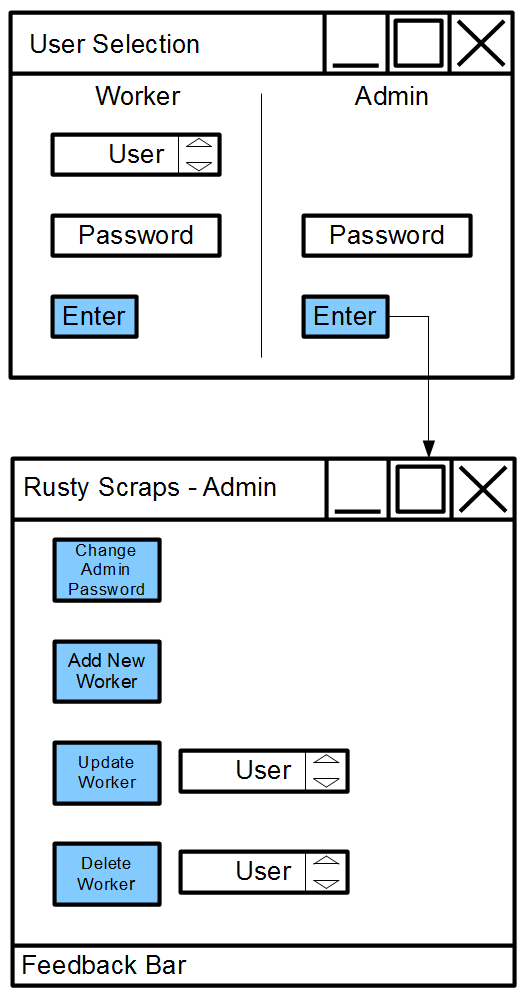
\includegraphics[width=\textwidth]{./Design/Images/AdminSelect.png}
\end{figure}

\begin{figure}[H]
    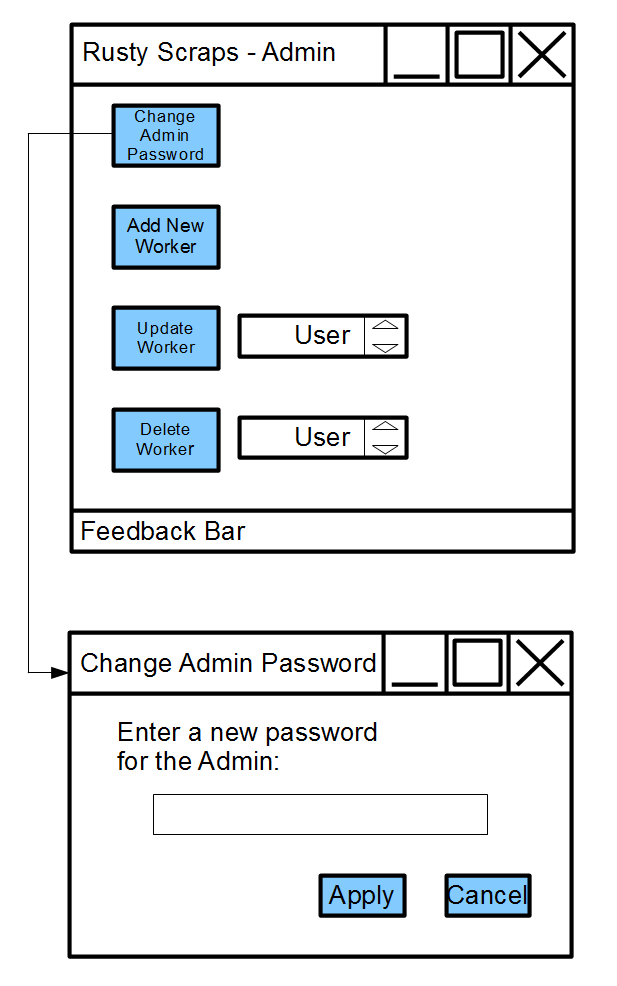
\includegraphics[width=\textwidth]{./Design/Images/ChangePassword.png}
\end{figure}

\begin{figure}[H]
    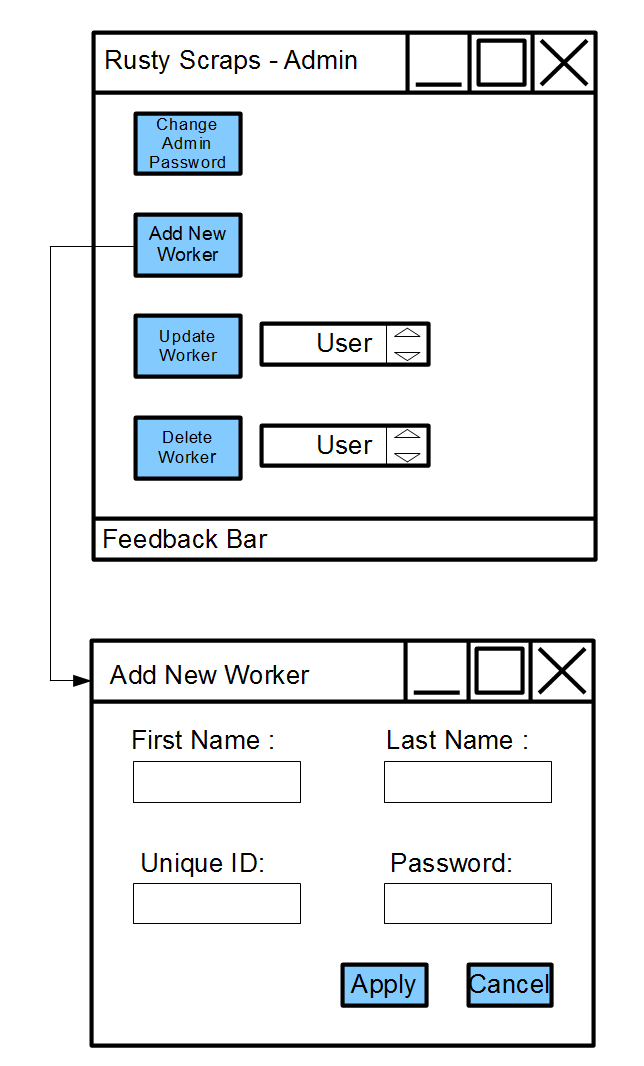
\includegraphics[width=\textwidth]{./Design/Images/AddWorker.png}
\end{figure}

\begin{figure}[H]
    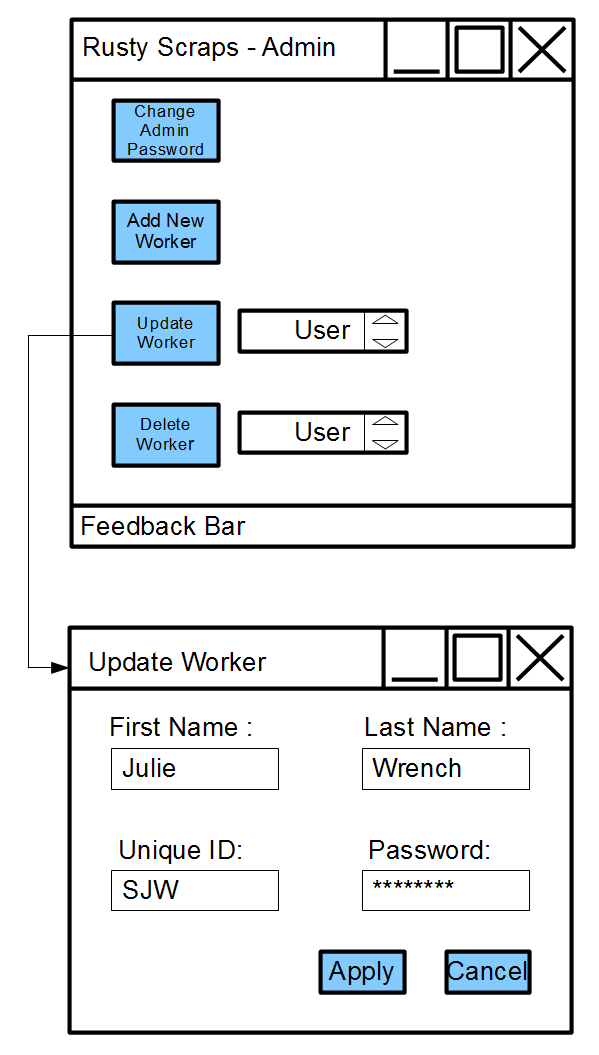
\includegraphics[width=\textwidth]{./Design/Images/UpdateWorker.png}
\end{figure}

\begin{figure}[H]
    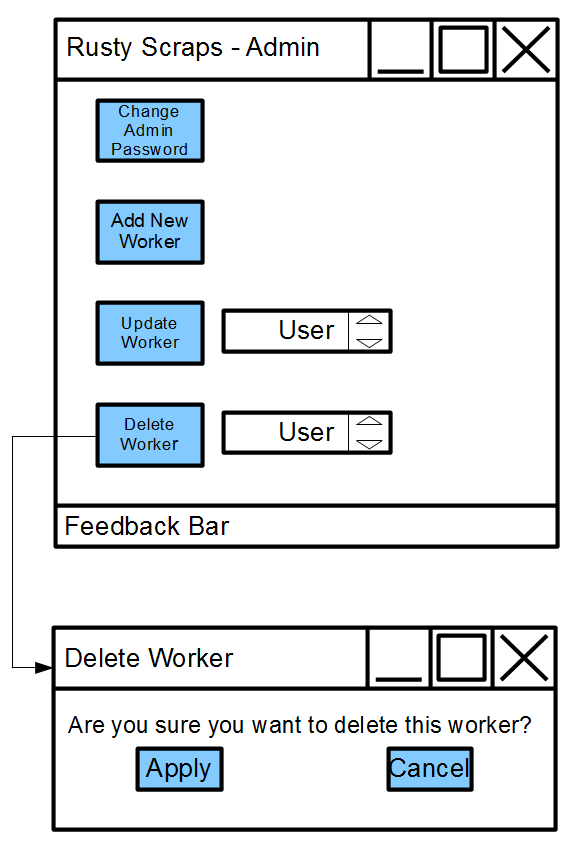
\includegraphics[width=\textwidth]{./Design/Images/DeleteWorker.png}
\end{figure}


\section{Hardware Specficiation}

The program will run on a reasonably modern Dell desktop computer, with 1080p monitor and accessories, running Windows 7 Home Edition. 8GBs of DDR3 RAM, an i5 Intel processor, and a AMD video card.This system uses a traditional mouse and keyboard as a input system. Choices will be made by using the mouse to click buttons, and data is inputted by typing on the keyboard. The screen resolution provides plenty of space for a large GUI, if such a size is required. The program will be stored on the computer's hard drive (500Gbs), which will provide plenty of space for the program and any data that gets recorded over the years.


\section{Definition of Data Requirements}


\subsection{Data Dictionary}

\begin{tabular}{|p{3.25cm}|p{1.5cm}|p{1.75cm}|p{3cm}|p{3.5cm}|}
	\hline
	\textbf{Data Name} & \textbf{Data Type} & \textbf{Data Length} & \textbf{Validation} & \textbf{Example} \\ \hline
	{DonationCode} & {String} & {7 characters} & {Allowed Characters, Range Check, Format Check} & {D123456} \\ \hline
	{Date} & {String} & {8 characters} & {Allowed Characters, Range Check} & {21/11/01} \\ \hline
	{ItemDescription} & {String} & {0 - 30 characters} & {Range Check} & {"A leather chair} \\ \hline
	{ItemPrice} & {Float} & {1 - 6 numbers} & {Allowed Character, Range Check, Format Check} & {54.32} \\ \hline
	{ItemCategory} & {Interger} & {1 - 2 numbers } & {Allowed Character, Range Check} & {5} \\ \hline
	{ItemCategoryDescription} & {String} & {0 - 15 characters} & {Table Look Up Check} & {"Furniture"} \\ \hline
	{ItemQualityCheck} & {Boolean} & {1 bit} & {Table Look Up Check} & {TRUE} \\ \hline
	{ItemCode} & {String} & {7 characters} & {Allowed Characters, Range Check, Format Check} & {I456789} \\ \hline
	{ItemStatus} & {String} & {4 -5 characters} & {Table Look Up Check} & {Store} \\ \hline
	{DonatorID} & {String} & {7 characters} & {Allowed Characters, Range Check} & {R654321} \\ \hline
	{DonatorFirstName} & {String} & {0 - 30 character} & {Range Check} & {"Wendy"} \\ \hline
	{DonatorLastName} & {String} & {0 - 30 character} & {Range Check} & {"Huddon"} \\ \hline
	{DonatorAddress1} & {String} & {0 - 30 character} & {Range Check} & {"2 Not Lane"} \\ \hline
	{DonatorAddress2} & {String} & {0 - 30 character} & {Range Check} & {"Flat 20C"} \\ \hline
	{DonatorCity} & {String} & {0 - 30 character} & {Range Check} & {"Lindun"} \\ \hline
	{DonatorCounty} & {String} & {0 - 30 character} & {Range Check} & {"Combrudgeshore"} \\ \hline
	{DonatorPostCode} & {String} & {0 - 7 character} & {Range Check} & {"SG3 78U"} \\ \hline
	{DonatorContact} & {String} & {0 - 30 character} & {Allowed Characters} & {"0147822673"} \\ \hline
	{StaffFirstName} & {String} & {0 - 30 character} & {Range Check} & {"Wiggy"} \\ \hline
	{StaffLastName} & {String} & {0 - 30 characters} & {Range Check} & {"Wog"} \\ \hline
	{StaffID} & {String} & {3 characters} & {Allowed Characters} & {"SWW"} \\ \hline
\end{tabular}


\subsection{Identification of appropriate storage media}
The hard drive of the computer that will be used with the program shall be appropriate for storing the program.

\section{Database Design}


\subsubsection{ER Diagrams}

\begin{figure}[H]
    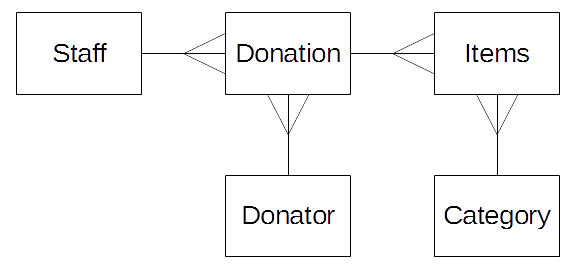
\includegraphics[width=\textwidth]{./Design/Images/ERDiagram.png}
\end{figure}

\subsubsection{Entity Descriptions}

Staff(\underline{StaffID},StaffFirstName,StaffLastName)
Category(\underline{ItemCategory},ItemCategoryDescription)
Item(\underline{ItemCode},ItemDescription,ItemPrice,\textit{ItemCategory},ItemQualityCheck,ItemStatus)
Donator(\underline{DonatorID},DonatorFirstName,DonatorLastName,DonatorAddress1,DonatorAddress2,
		DonatorCity,DonatorCounty,DonatorPostCode,DonatorContact)
Donation(\underline{DonationCode},\textit{ItemCode},\textit{DonatorID},\textit{StaffID},Date)

\subsubsection{1NF to 3NF}

Primary Key 		= *
Composite Key	= \%
Foreign Key		= \# 
\begin{center}
    \begin{tabular}{|p{4.5cm}|p{4.5cm}|}
	\hline
	\multicolumn{2}{|c|}{UNF} \\
	\hline
	\textbf{DonationCode} & \textbf{DonatorLastName} \\ \hline
	\textbf{Date} & \textbf{DonatorAddress1} \\ \hline
	\textbf{ItemDescription} & \textbf{DonatorAddress2} \\ \hline
	\textbf{ItemPrice} & \textbf{DonatorCity} \\ \hline
	\textbf{ItemCategory} & \textbf{DonatorCounty} \\ \hline
	\textbf{ItemCategoryDescription} & \textbf{DonatorPostCode} \\ \hline
	\textbf{ItemQualityCheck} & \textbf{DonatorDontact} \\ \hline
	\textbf{ItemCode} & \textbf{StaffFirstName} \\ \hline
	\textbf{ItemStatus} & \textbf{StaffLastName} \\ \hline
	\textbf{DonatorID} & \textbf{StaffID} \\ \hline
	\textbf{DonatorFirstName} & \textbf{}\\ \hline
    \end{tabular}
\end{center}
	
\begin{center}
    \begin{tabular}{|p{4.5cm}|p{4.5cm}|}
	\hline
	\multicolumn{2}{|c|}{1NF} \\
	\hline
	\textbf{Repeating} & \textbf{Non-Repeating} \\ \hline
	{ItemDescription} & {DonationCode *} \\ \hline
	{ItemPrice} & {Date} \\ \hline
	{ItemCategory} & {DonatorID} \\ \hline
	{ItemCategoryDiscription} & {DonatorFirstName} \\ \hline
	{ItemQualityCheck} & {DonatorLastName} \\ \hline
	{ItemCode *} & {DonatorAddress1} \\ \hline
	{ItemStatus} & {DonatorAddress2} \\ \hline
	{DonationCode \%} & {DonatorCity} \\ \hline
	{} & {DonatorCounty} \\ \hline
	{} & {DonatorPostCode} \\ \hline
	{} & {DonatorContact} \\ \hline
	{} & {StaffFirstName} \\ \hline
	{} & {StaffLastName} \\ \hline
	{} & {StaffID} \\ \hline
    \end{tabular}
\end{center}

\begin{center}
\begin{tabular}{|p{4.5cm}|p{4.5cm}|}
\hline
\multicolumn{2}{|c|}{2NF}                                       \\ \hline
DonationCode*     & \multicolumn{1}{l|}{ItemDescription}         \\
Date             & \multicolumn{1}{l|}{ItemPrice}               \\
DonatorID        & \multicolumn{1}{l|}{ItemCategory}            \\
DonatorFirstName & \multicolumn{1}{l|}{ItemCategoryDescription} \\
DonatorLastName  & \multicolumn{1}{l|}{ItemQualityCheck}        \\
DonatorAddress1  & \multicolumn{1}{l|}{ItemCode*}                \\
DonatorAddress2  & \multicolumn{1}{l|}{ItemStatus}              \\
DonatorCity      & \multicolumn{1}{l|}{}                        \\ \cline{2-2} 
DonatorCounty    &                                              \\
DonatorPostCode  &                                              \\
DonatorContact   &                                              \\
StaffFirstName   &                                              \\ \cline{2-2} 
StaffLastName    & \multicolumn{1}{l|}{ItemCode *}                \\
StaffID          & \multicolumn{1}{l|}{DonationCode *}            \\ \hline
\end{tabular}
\end{center}

\begin{center}
\begin{tabular}{|p{4.5cm}|p{4.5cm}|}
\hline
\multicolumn{2}{|c|}{3NF}                                                             \\ \hline
\multicolumn{1}{|l|}{DonatorID *}      & \multicolumn{1}{l|}{ItemCode *}              \\
\multicolumn{1}{|l|}{DonatorFirstName} & \multicolumn{1}{l|}{ItemDescription}         \\
\multicolumn{1}{|l|}{DonatorLastName}  & \multicolumn{1}{l|}{ItemPrice}               \\
\multicolumn{1}{|l|}{DonatorAddress1}  & \multicolumn{1}{l|}{ItemCategory \#}         \\
\multicolumn{1}{|l|}{DonatorAddress2}  & \multicolumn{1}{l|}{ItemQualityCheck}        \\
\multicolumn{1}{|l|}{DonatorCity}      & \multicolumn{1}{l|}{ItemStatus}              \\ \cline{2-2} 
\multicolumn{1}{|l|}{DonatorCounty}    &                                              \\ \cline{2-2} 
\multicolumn{1}{|l|}{DonatorPostCode}  & \multicolumn{1}{l|}{ItemCategory *}          \\
\multicolumn{1}{|l|}{DonatorContact}   & \multicolumn{1}{l|}{ItemCategoryDescription} \\ \hline
                                       &                                              \\ \hline
\multicolumn{1}{|l|}{StaffID *}        & \multicolumn{1}{l|}{DonationCode*}           \\
\multicolumn{1}{|l|}{StaffFirstName}   & \multicolumn{1}{l|}{ItemCode \#}             \\
\multicolumn{1}{|l|}{StaffLastName}    & \multicolumn{1}{l|}{DonatorID \#}            \\ \cline{1-1}
\multicolumn{1}{l|}{}                  & \multicolumn{1}{l|}{StaffID \#}              \\
\multicolumn{1}{l|}{}                  & \multicolumn{1}{l|}{Date}                    \\ \cline{2-2} 
\end{tabular}
\end{center}

\section{Security and Integrity of the System and Data}

\subsection{Security and Integrity of Data}
The database will hold details about the donators and staff. Due to this, the system falls under regulation from the Data Protection Act (1998), requiring the data be secured in such a way that non-permitted people may have access to it. The data will also require updating in accordance to changes with the people's whos' information is stored by the system.

\subsection{System Security}
A password system will be implimented, allowing only staff to get access to the program. Passwords will not be stored in plain text.